\documentclass[11pt]{article}
% arXiv: force pdflatex output (PNG figures require it). Keyed on \pdftexversion
% (pdfTeX-only) so it is a true no-op under XeTeX/tectonic.
\ifdefined\pdftexversion \pdfoutput=1 \fi

\usepackage[margin=1in]{geometry}
\usepackage{graphicx}
\usepackage{amsmath}
\usepackage{booktabs}
\usepackage{textcomp}   % \textdegree, for arXiv's pdflatex
\usepackage{xcolor}
\usepackage[hidelinks]{hyperref}
\usepackage{caption}
\usepackage{parskip}

% Figures resolve either from a local figures/ dir (the arXiv submission bundle)
% or from the repo's eval/ tree (an in-repo build). Bare filenames below.
\graphicspath{{figures/}{../eval/pit/figures/}}

\newcommand{\rstar}{r^{\star}}
\newcommand{\code}[1]{\texttt{#1}}

\title{\textbf{Judge vs.\ React:\\ dissociating perception from timing in VLM reflex control}}
\author{Josh Simnitt\\ \small\texttt{jsimnitt@gmail.com}}
\date{2026}

\begin{document}
\maketitle

\begin{abstract}
A vision-language-model (VLM) agent that must time a single action in a
first-person scene can fail two ways that existing game benchmarks cannot pull
apart: it can misjudge the scene (perception), or judge correctly but act too
late (timing). We build a minimal, parametric first-person pit-jump task that
reduces an episode to one correct decision, and use it to dissociate the two
axes. We show (i) a \textbf{same-decision flip} --- the \emph{identical} correct
decision clears the pit when the world is paused and fails in real time; (ii) a
\textbf{quantitative timing law} --- success collapses at a sharp threshold in
the dimensionless ratio $r = \text{latency} / \text{action-window}$, located
near $r \approx 1$ (logistic fit $\rstar = 1.17$ on the oracle apparatus), with
latency varied \emph{independently of judgment quality}; (iii)
\textbf{action-repeat does not rescue it}; and (iv) the boundary is a
\textbf{law, not a quirk of one task} --- a second reflex task in a different
modality (rotational aiming) collapses onto the same $r \approx 1$ transition
($\rstar = 0.98$). Measuring five real vision models on the task, \textbf{all
land past $\rstar$} --- hosted frontier models at $r \approx 4$--$6$, local open
VLMs at $r \approx 31$--$47$ --- so none can act inside the window in real time,
yet the same decisions succeed when the world is paused. The framing implies
that pausable/turn-based deployment converts a slow-but-accurate VLM from
failing to viable, and that ``VLMs are too slow to play games'' is partly an
artifact of the time regime they are benchmarked in.
\end{abstract}

\section{Introduction}

When a vision-language model plays a real-time game and walks into a pit, the
post-mortem is ambiguous. Did it fail to \emph{see} that a jump was needed
(perception), or did it see correctly and \emph{act too late} (timing)?
Aggregate game benchmarks --- score, win rate, levels cleared --- fold these two
failures into one number, so ``the VLM is bad at this game'' can mean either,
and usually means some unknown mix. The two have opposite fixes: a perception
failure wants a better model; a timing failure wants a slower clock. Conflating
them is why ``VLMs are too slow to play games'' is repeated as though it were a
single fact.

Our move is isolation. We reduce an episode to \emph{one} correct decision --- a
first-person pit the player auto-walks toward, where the only choice is
\emph{when} to jump --- so that on any given run exactly one of the two failures
can occur, and we can say which. The apparatus is deterministic and headless,
and it injects a control delay $D$ (a decision made at tick $t$ is applied at
$t{+}D$), which lets us vary \emph{lateness} completely independently of
\emph{judgment quality}: a perfect-judgment oracle still fails if its action
lands too late.

That isolation yields four results, presented most striking first:

\begin{itemize}
  \item \textbf{S2 (dissociation):} the same correct decision succeeds when the
    world is paused and fails in real time, isolating latency from perception on
    a single decision.
  \item \textbf{S1 (timing law):} success collapses at a sharp threshold in
    $r = \text{latency}/\text{window}$ near $1$, with latency varied
    independently of judgment quality.
  \item \textbf{S3 (no cheap fix):} action-repeat does not rescue the transition
    (and modestly worsens it --- larger $k$ fails at lower $r$).
  \item \textbf{S4 (generality):} a second reflex task in a different modality
    (rotational aiming) collapses onto the same $r \approx 1$ boundary
    ($\rstar = 0.98$) --- the law is not specific to the pit.
\end{itemize}

Separately, on the perception axis, a blind vision model \emph{can} judge the
jump from a single frame, and obscuring the depth cue (fog) collapses that
judgment to chance --- at zero delay, i.e.\ independent of the timing axis.

\section{Related work}

Five works are closest; we differentiate from each.

\begin{itemize}
  \item \textbf{OmniGameArena} (Lin et al., 2026, arXiv:2606.09826) --- has
    paused (PDQ) vs.\ latency-controlled real-time (LCRT) clock modes, but only
    as \textbf{aggregate whole-game} comparisons; no ratio transition, no
    single-decision flip, no action-repeat test. We add all three.
  \item \textbf{VideoGameBench} (Zhang et al., 2025, arXiv:2505.18134) ---
    ``Lite'' (paused) vs.\ real-time; names the stale-action mechanism but
    leaves perception confounded (``it's not just latency''). We resolve exactly
    that confound by isolating one decision.
  \item \textbf{``Win Fast or Lose Slow''} (Kang et al., NeurIPS 2025,
    arXiv:2505.19481) --- owns the latency--quality tradeoff, but its latency
    lever is quantization/model-size, which \emph{also} degrades quality, and
    its $\approx$200\,ms point is an environment action-rate cap, not a
    task-window threshold. Our $r \approx 1$ collapse
    varies latency \textbf{independently} of the model --- the apparatus injects
    control delay $D$ with the policy fixed.
  \item \textbf{BLINK} (Fu et al., ECCV 2024, arXiv:2404.12390) --- canonical
    ``MLLMs fail at depth,'' but static MCQ. Ours is interactive, parametric,
    oracle-normalized.
  \item \textbf{Ramstedt \& Pal, ``Real-Time RL''} (NeurIPS 2019,
    arXiv:1911.04448) [+ ``At Human Speed,'' arXiv:1810.07286] --- the RL parent
    of the real-time/delay result (monotone degradation for learned policies).
    We locate an $r \approx 1$ boundary for \emph{pausable VLM agents} and show
    turn-based deployment crosses it.
\end{itemize}

We explicitly do \textbf{not} claim to be first to study the latency--quality
tradeoff (Win Fast) nor first to isolate timing from competence in the aggregate
(Real-Time Deadlines, arXiv:2601.13206; OmniGameArena). Our claim is the
single-decision flip plus the quality-controlled ratio law, and its generality
across a second task.

\section{Task and apparatus}

A first-person raycaster. The player auto-walks toward a pit; the only decision
is \emph{when} to jump. Knobs: pit width (sets the action-window $W$),
fog/visibility (perception), approach speed $v$, seed. The sim is deterministic
and headless; control delay $D$ (ticks) is \textbf{injected} --- a decision made
at tick $t$ is applied at $t{+}D$ --- so $D$ is an independent variable
decoupled from wall-clock. Real per-model latency $L$ is measured separately
(timed calls) and mapped to the $r$ axis via $L/\text{tick}$. An oracle policy
(true pit distance) is the perfect-judgment ceiling.

\paragraph{Ground-truth label.} \code{in\_window} $=$ whether a delay-0 takeoff
at the decision position clears, computed from the sim's \emph{own} dynamics
(not an analytic approximation), so \code{in\_window} exactly predicts
\code{cleared} at $D{=}0$. The action window is $W = w_{hi} - w_{lo}$ with
$w_{lo}, w_{hi}$ derived by simulating takeoffs; for pit widths beyond the jump
reach the window is empty ($W \le 0$, unclearable) and those configs are
excluded from fits (reported, not silently dropped).
\[
  r = \frac{v \cdot D}{W}\ \text{(oracle sweep)}
  \qquad\text{or}\qquad
  r = \frac{v \cdot (L/\text{tick})}{W}\ \text{(real-model placement).}
\]

\section{Results}

\subsection{Timing law (S1)}

Sweeping $D$ for each pit width (each a different $W$) and pooling against $r$,
the clear/fail outcomes \textbf{collapse onto a single transition near
$r \approx 1$}; a logistic fit gives $\rstar = 1.17$ (420/1680 empty-window rows
excluded). Because the delay grid is discrete, the data bracket the edge rather
than pinpoint it: the last clearing configuration lies at $r = 1.04$ and the
first failure at $r = 1.30$; $\rstar = 1.17$ is the logistic midpoint of that
gap. The transition is razor-sharp because the oracle is deterministic; a
stochastic VLM would smooth it into a psychometric curve. The slight offset
above $1.0$ is physical: a jump firing on the same tick can take off from just
past the pit's near edge, extending tolerance marginally beyond the nominal
window --- hence clears observed at $r = 1.04$.

\begin{figure}[h]
  \centering
  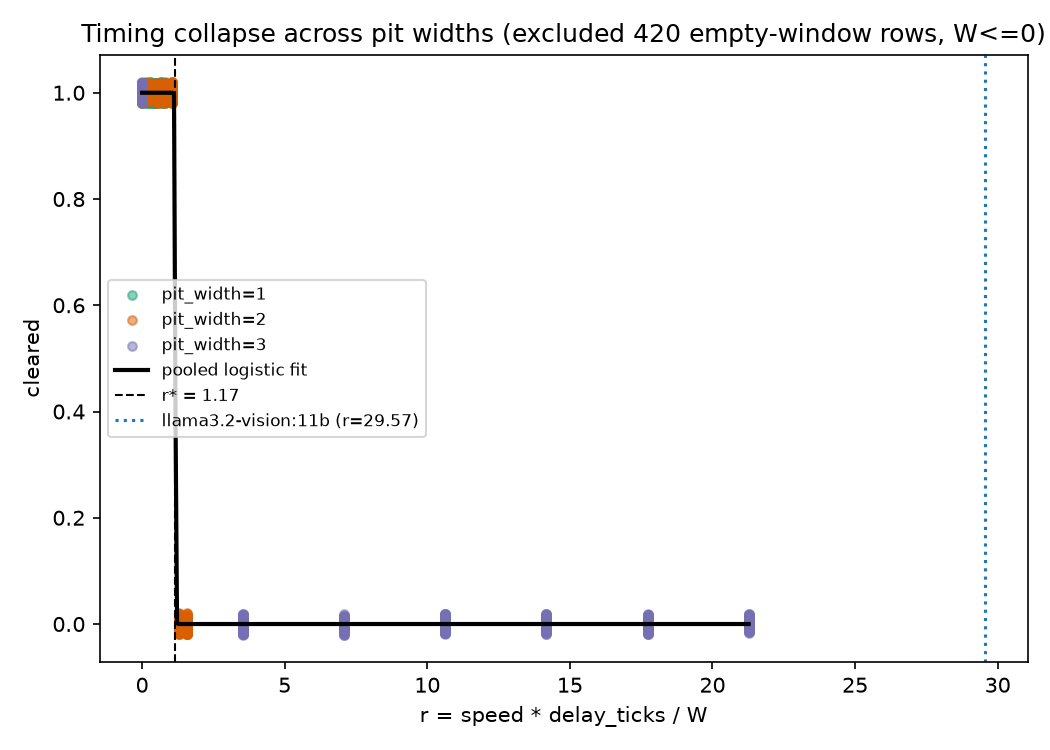
\includegraphics[width=0.72\linewidth]{fig_timing.png}
  \caption{S1. Clear/fail collapses onto a single transition near $r \approx 1$
  across pit widths (pooled logistic fit $\rstar = 1.17$).}
\end{figure}

\paragraph{Real models all land past $\rstar$.} Because the decision cost is
exactly $r = L / T_{\text{window}}$, where the window is open for
$T_{\text{window}} = (W/v)\cdot\text{tick} = 257\,\text{ms}$ at pit width 2
($W = 1.078$, $v = 0.07$), the $\rstar$ boundary sets a \textbf{maximum
tolerable decision latency of $\rstar\cdot T_{\text{window}} \approx 300\,$ms}.
We timed five vision models on the identical 20-frame decision battery, in each
model's \emph{fastest} single-call configuration ($n = 20$ each):

\begin{table}[h]
  \centering
  \caption{Measured per-model decision latency (median of $n = 20$ single-frame
  calls, fastest configuration) against the 257\,ms window at pit width 2.}
  \begin{tabular}{lrr}
    \toprule
    Model & Median $L$ & $r = L / \text{window}$ \\
    \midrule
    Haiku 4.5 (hosted API)        & 0.95\,s  & $\approx 4$ \\
    Sonnet 4.6 (hosted API)       & 1.45\,s  & $\approx 6$ \\
    Opus 4.8 (hosted API)         & 1.53\,s  & $\approx 6$ \\
    Qwen2.5-VL 7B (local)         & 7.9\,s   & $\approx 31$ \\
    llama3.2-vision 11B (local)   & 12.1\,s  & $\approx 47$ \\
    \bottomrule
  \end{tabular}
\end{table}

\textbf{None clear the 300\,ms budget.} Even the \emph{fastest hosted frontier
model} is $\sim$4$\times$ too slow, and local open VLMs are 30--47$\times$. This
is the concrete version of ``VLMs are too slow to play games'': the whole
measured field would need the world \textbf{paused, or slowed 4--47$\times$}, to
act inside the window --- and the gap is a property of the \emph{time regime},
not the model, since $r$ here is $L/\text{window}$ with judgment held out
entirely. The hosted numbers are a model's best case (this fast config uses no
extended thinking; any more deliberate configuration is only slower); local
latency is on-device --- a real, reproducible closed-loop number.

A closed-loop episode (blocking mode) confirms the local model is non-viable,
though the two failure modes should be separated: \code{llama3.2-vision} also
\emph{fails perception} --- it answered JUMP on all 20 frames (no depth
discrimination), so in blocking mode it jumps at tick 0 from $x \approx 2.6$
(far from the pit at $x = 10$) and falls. The latency result is the
axis-independent point: $r > \rstar$ dooms even a model that judges correctly,
the moment the world is allowed to run in real time.

\begin{figure}[h]
  \centering
  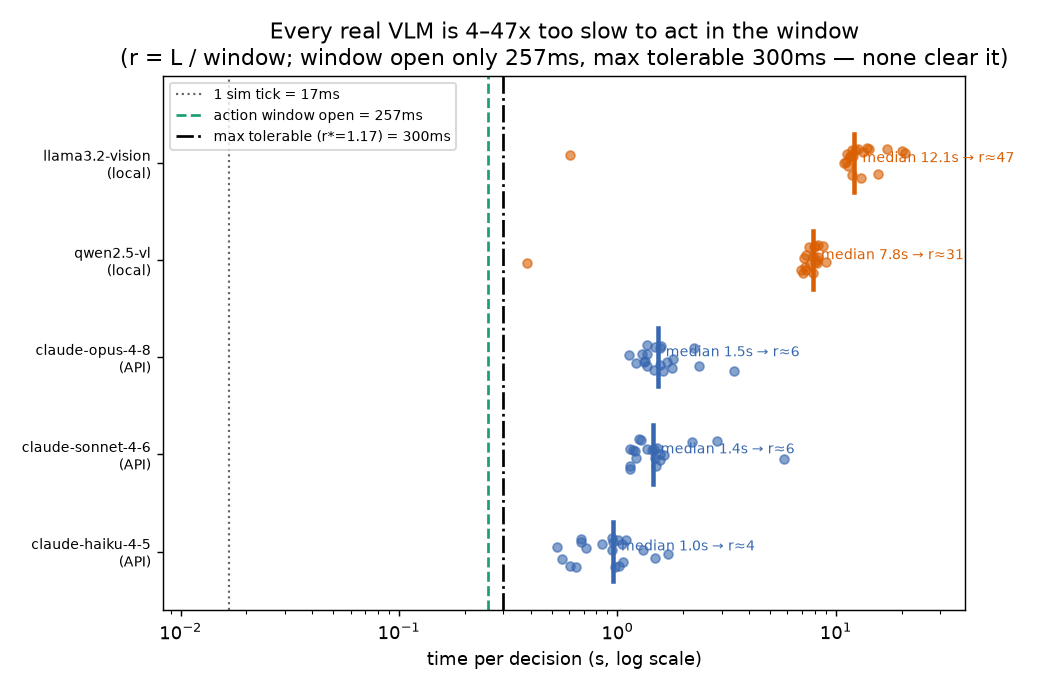
\includegraphics[width=0.86\linewidth]{fig_latency.png}
  \caption{Real per-model decision latency vs.\ the time budget. Hosted
  Haiku/Sonnet/Opus ($r \approx 4$--$6$) and local Qwen/llama3.2-vision
  ($r \approx 31/47$); all past the $\approx$300\,ms max-tolerable budget.}
\end{figure}

\subsection{Same-decision flip (S2)}

Restricting to oracle-correct decisions (\code{in\_window} $= 1$), the
\textbf{identical} decision clears with probability \textbf{1.00 at $D = 0$} and
\textbf{0.11 once $D$ exceeds the window} ($r > 1$). The decision is the same
(same \code{decision\_x}, delay-independent); only execution timing changed.
This isolates latency from perception directly. (These are unique configs, not
raw rows: the oracle emits $60\times$ fog/seed duplicates; the ``late''
condition is 9 unique configs, 1 of which still clears, giving 0.11.)

\begin{figure}[h]
  \centering
  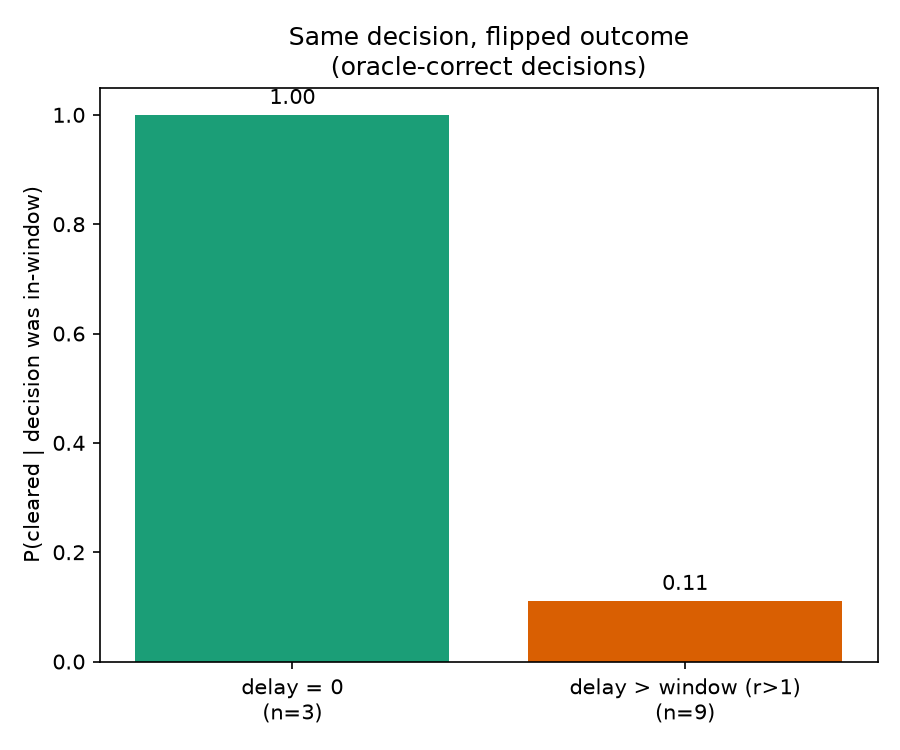
\includegraphics[width=0.66\linewidth]{fig_flip.png}
  \caption{S2. The same correct decision clears 1.00 paused and 0.11 once delay
  pushes it past the window.}
\end{figure}

\subsection{Action-repeat does not rescue (S3)}

Holding a decision across $k$ frames does not rescue the timing failure --- and
in fact modestly \textbf{worsens} it. Measured $\rstar$ vs.\ $k$ (fixed pit
width): $k{=}1 \to 1.10$, $k{=}2,4 \to 0.97$, $k{=}8,16 \to 0.71$. Consulting
the policy less often means a decision lands staler (up to $k{-}1$ ticks later
than ideal), so the transition moves to \emph{lower} $r$ (fails earlier), not
higher. Action-repeat is a compute/cost lever, not a latency fix. (This sweep is
at a single pit width; extending it across widths to confirm the direction is
general is future work.)

\begin{figure}[h]
  \centering
  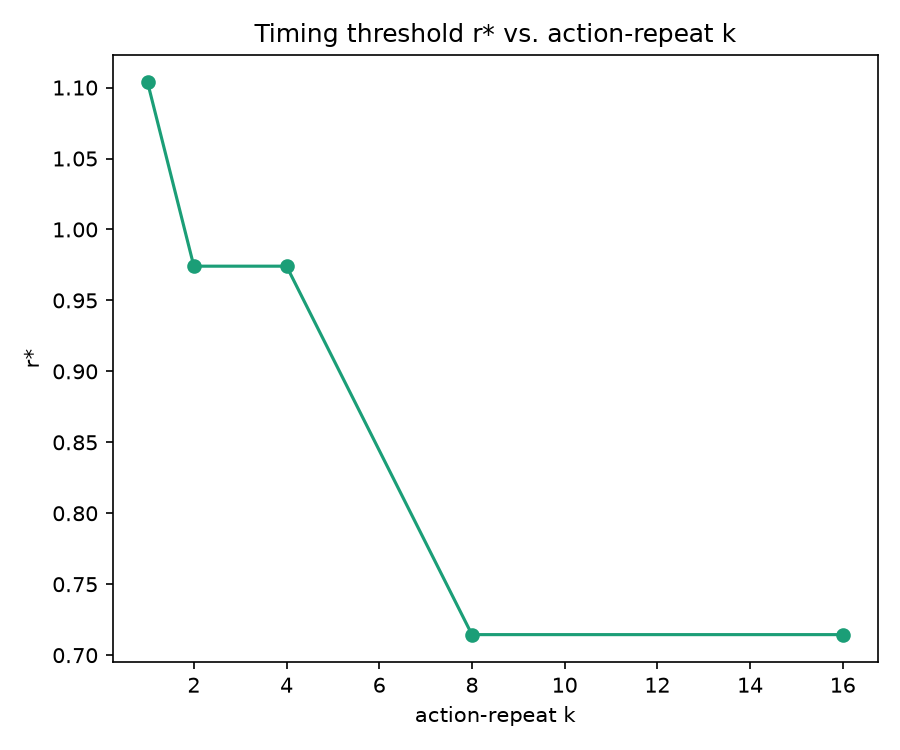
\includegraphics[width=0.66\linewidth]{fig_repeat.png}
  \caption{S3. Action-repeat does not rescue the transition; larger $k$ fails at
  lower $r$.}
\end{figure}

\subsection{Perception axis (dissociation)}

A capable vision model \emph{can} judge the jump from a single frame, and fog
collapses it. We rendered standing decision frames across approach positions at
two visibility levels and had \textbf{four blind vision models} --- three Claude
models (Haiku 4.5, Sonnet, Opus) and one local open VLM (\code{qwen2.5-vl:7b}
via Ollama) --- each shown only the image (no coordinates, window, or labels;
identical seed-42 shuffled frame set) call JUMP or WAIT on each; we score each
call against the ground-truth window. Judgment accuracy at zero delay ($n = 10$
frames per model per condition):

\begin{table}[h]
  \centering
  \caption{Blind single-frame judgment accuracy at zero delay
  ($n = 10$ frames per model per condition; exact counts shown).}
  \begin{tabular}{lccc}
    \toprule
    Model & Clear (fog=0) & Foggy (fog=1) & Fog effect \\
    \midrule
    Opus                    & \textbf{90\%} (9/10) & 50\% (5/10, chance) & $\mathbf{-40}$ pts \\
    Sonnet                  & 80\% (8/10)          & 50\% (5/10, chance) & $\mathbf{-30}$ pts \\
    Qwen2.5-VL 7B (local)   & 60\% (6/10)          & 60\% (6/10)         & 0 \\
    Haiku 4.5               & 40\% (4/10)          & 40\% (4/10)         & 0 \\
    \bottomrule
  \end{tabular}
\end{table}

Two things fall out. \textbf{(1) With a clear depth cue, judgment scales with
model capability} --- Opus 90\%, Sonnet 80\%, Qwen 60\%, Haiku 40\%. \textbf{(2)
The fog collapse appears only in the models that actually read depth.} Opus and
Sonnet drop to chance under fog, and each \textbf{missed every in-window frame}
(0/5): they reported no distinguishable pit band even up close, never committed,
and would fall. The two weak judges show \textbf{no fog effect at all} --- but
for opposite-looking reasons that are really the same reason: Haiku sits at
floor (it fell back on a frame-order heuristic the shuffle nullifies), and Qwen
is strongly \emph{JUMP-biased} (it answered JUMP on 18/20 frames, clearing all
in-window frames but also most out-of-window ones). Neither is using the depth
cue in the first place, so neither has any perception to lose when fog removes
it. The fog collapse is a \textbf{signature of genuine depth reading}, present
exactly where clear-condition accuracy is high. At $n = 10$ frames per cell the
per-model contrasts are directional rather than individually significant
(Fisher exact, clear vs.\ fog: Opus $p = 0.14$, Sonnet $p = 0.35$; pooled
Opus$+$Sonnet $17/20$ vs.\ $10/20$, $p = 0.04$) --- it is the coherence of the
pattern across four models, not any single cell, that carries the claim.

This is the perception half of the dissociation: a model that judges well with a
clear depth cue drops to chance when fog obscures the pit's distance ---
\textbf{at zero delay}, i.e.\ independent of the timing axis. Together,
perception and timing are separable failure axes on one task. (Caveat: the
Claude judges run via a subagent path, not a controlled API benchmark; the local
VLM is a real keyless run. Judges are blinded to coordinates and labels but not
to the task; the local VLMs' latencies place them on the timing axis at
$r \approx 31$ (Qwen) and $r \approx 47$ (llama3.2-vision).)

\begin{figure}[h]
  \centering
  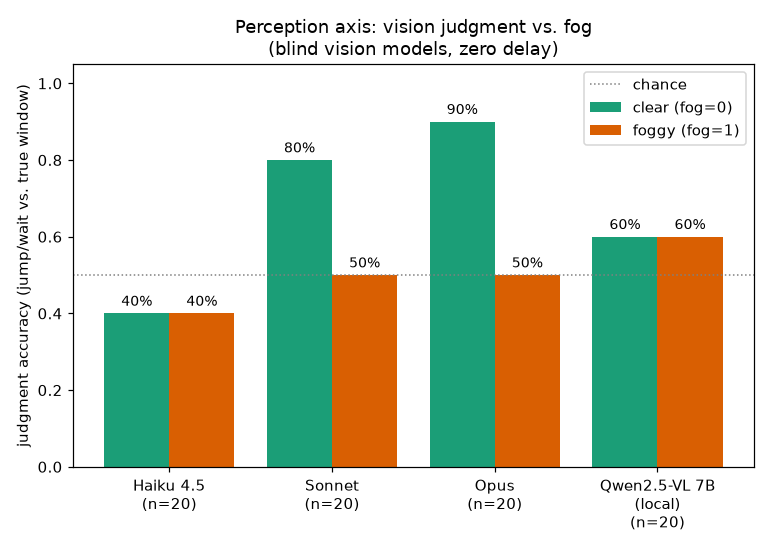
\includegraphics[width=0.72\linewidth]{fig_perception.png}
  \caption{Perception axis. Fog collapses judgment to chance only for the
  depth-reading models (Opus, Sonnet); JUMP-biased/floor judges show no fog
  effect.}
\end{figure}

\subsection{Generality (S4)}

Is $r \approx 1$ specific to jump-timing, or a property of \emph{any}
act-in-a-window reflex? We built a second task in a different modality: a
\textbf{sweeping-aim} task. The player rotates in place at constant angular speed
$\omega$; a target subtends an angular window $[\theta - h, \theta + h]$ (width
$2h$); the single decision is \emph{fire}, and a control delay $D$ rotates the
aim $\omega D$ further before the shot lands --- overshoot if it exceeds the
window. By construction the dimensionless cost is $r = \omega D / (2h)$, the
exact angular analog of the pit's $vD/W$. The aim episode is pure kinematics and
emits the same schema, so the \emph{identical} fit machinery applies.

Sweeping $D$ across five target widths (4.6\textdegree--13.8\textdegree) and
pooling against $r$, the hit/miss outcomes \textbf{collapse onto the same
transition near $r \approx 1$} --- logistic fit $\rstar = 0.98$ ($n = 205$). A
translational jump task and a rotational aiming task, sharing nothing but the
``act inside a window that your delay pushes you out of'' structure, land on the
\textbf{same boundary}. The small offset between the two $\rstar$ (pit 1.17, aim
0.98) is the oracles' firing phase: the pit's takeoff can extend just \emph{past}
the near edge (a hair above 1), while the aim fires just \emph{inside} the near
edge, forfeiting a sub-tick of tolerance (a hair below 1). The raw step edges
show exactly this: the pit's last clear lands at $r = 1.04$ (past the nominal
edge), while the aim's last hit is at $r = 0.96$ and its first miss at exactly
$r = 1.00$. Both are the same order-unity law. This is the result that makes $r \approx 1$ a \emph{law} rather
than a fact about one pit.

\begin{figure}[h]
  \centering
  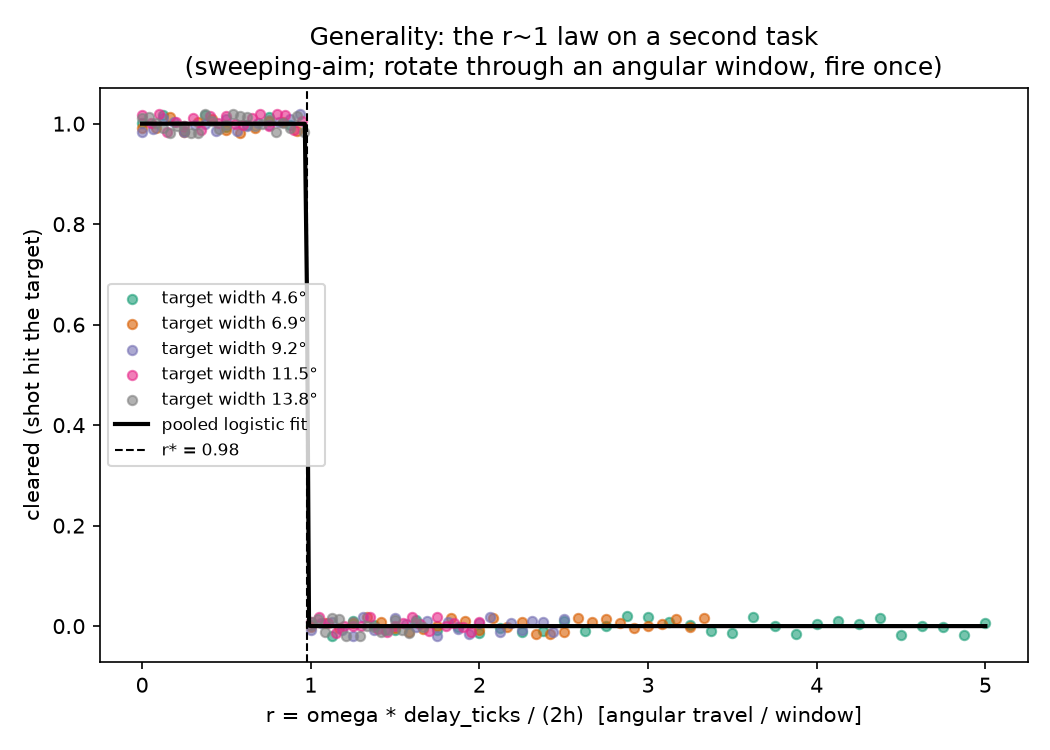
\includegraphics[width=0.72\linewidth]{fig_aim.png}
  \caption{S4. The same $r \approx 1$ collapse on a rotational aiming task
  ($\rstar = 0.98$, 5 target widths).}
\end{figure}

\section{Discussion}

The two failure axes have opposite fixes, and the framing makes the requirement
quantitative. A perception failure wants a better model: no amount of extra
time helps a judge that reports no distinguishable pit band under fog. A timing
failure wants a slower clock: a model is viable exactly when
$r = L / T_{\text{window}} < \rstar \approx 1$, so a deployment can cross the
boundary by pausing the world ($r \to 0$), slowing it (raising
$T_{\text{window}}$), or cutting latency --- and the measured field needs
4--47$\times$ on the latter two. The practical reading is that pausable or
turn-based deployment converts every slow-but-accurate model we measured from
failing to viable, with no change to the model; conversely, a real-time
benchmark score is a product of judgment \emph{and} time regime, and ``VLMs are
too slow to play games'' is partly a fact about the clock they are handed.

\section{Limitations}

\begin{itemize}
  \item \textbf{The timing \emph{sweep} is oracle-only.} Determinism makes the
    transition a sharp step, not a smooth psychometric curve; a stochastic
    real-model sweep would give the noisy version. The \textbf{latency axis is
    real}, though: five models are measured directly, all landing past $\rstar$
    (hosted $r \approx 4$--$6$, local $r \approx 31$--$47$). Hosted latencies are
    network- and load-dependent and local ones are hardware-specific, but each
    is a real measured decision latency, not a stand-in. What is not yet done is
    a real model swept \emph{through} the boundary (no model we measured lands
    near $r = 1$; the oracle alone maps the transition itself).
  \item \textbf{The perception axis} mixes three Claude judges (run via a
    subagent path, not a controlled API benchmark) with one real keyless local
    VLM (\code{qwen2.5-vl:7b}), at $n = 10$ frames per condition --- large
    enough for the cross-model pattern, too small for per-model significance
    (Fisher exact $p = 0.14$--$0.35$). The open VLMs are weak/biased judges --- Qwen is
    JUMP-biased (60\% clear, no fog effect) and \code{llama3.2-vision:11b} is
    always-JUMP (contributes latency only, not a perception point). A controlled,
    latency-timed multi-provider API sweep still needs a key.
  \item \textbf{No human baseline} --- the oracle stands in as the
    perfect-judgment ceiling. Human psychophysics is future work.
  \item \textbf{Two tasks, not many.} The $r \approx 1$ law now holds on two
    tasks in two modalities (translational jump, rotational aim), which is the
    difference between a fact and a law --- but both are single-decision reflex
    tasks in the same engine. Multi-decision and richer tasks are untested.
  \item \textbf{Deterministic-duplication caveat:} the oracle emits identical
    rows across fog/seed; reported counts are unique configs, and the sharp fit
    reflects zero per-episode noise.
\end{itemize}

\section{Future work}

A stochastic real-model sweep \emph{through} the boundary (engineering
$r \approx 1$ by widening the window or slowing the world, to trace the noisy
psychometric transition a real model produces); a multi-provider latency panel
(Gemini/GPT + more open VLMs); a human psychophysics arm; and more reflex tasks
(beyond the two here) to test how universal the $r \approx 1$ boundary is.

\section*{Reproducibility}

Code, data, and figure-generating scripts are at
\url{https://github.com/star7js/judge-vs-react}, under \code{eval/pit/}
(analysis and sweeps) and \code{raycaster/} (the deterministic sim, including
\code{--task aim} for the second task). The perception judgments
(\code{perception\_judgments.jsonl}, 80 rows across 4 models), per-decision
latencies (\code{vlm\_latency.jsonl}, 100 rows across 5 models), and the oracle
and aim sweeps are committed. The local-VLM paths (Ollama) and the Claude
subagent judges run without an API key; only the hosted-API latency numbers
required one.

\begin{thebibliography}{9}
  \bibitem{omnigamearena} M. Lin et al. \emph{OmniGameArena: A Unified UE5
    Benchmark for VLM Game Agents with Improvement Dynamics}.
    arXiv:2606.09826, 2026.
  \bibitem{videogamebench} A. L. Zhang, T. L. Griffiths, K. Narasimhan, O. Press.
    \emph{VideoGameBench: Can Vision-Language Models complete popular video
    games?} arXiv:2505.18134, 2025.
  \bibitem{winfast} H. Kang et al. \emph{Win Fast or Lose Slow: Balancing Speed
    and Accuracy in Latency-Sensitive Decisions of LLMs}. NeurIPS 2025,
    arXiv:2505.19481.
  \bibitem{blink} X. Fu et al. \emph{BLINK: Multimodal Large Language Models Can
    See but Not Perceive}. ECCV 2024, arXiv:2404.12390.
  \bibitem{realtimerl} S. Ramstedt, C. Pal. \emph{Real-Time Reinforcement
    Learning}. NeurIPS 2019, arXiv:1911.04448.
  \bibitem{athumanspeed} V. Firoiu, T. Ju, J. Tenenbaum. \emph{At Human Speed:
    Deep Reinforcement Learning with Action Delay}. arXiv:1810.07286, 2018.
  \bibitem{realtimedeadlines} N. K. R. Sehgal, S. C. Guntuku, L. Ungar.
    \emph{Real-Time Deadlines Reveal Temporal Awareness Failures in LLM
    Strategic Dialogues}. arXiv:2601.13206, 2026.
\end{thebibliography}

\end{document}
